\documentclass[./../main.tex]{subfiles}
\graphicspath{{img/}}
\begin{document}
	\begin{exercise}
		Este ejercicio se desdobla en dos, si no deseas hacer la parte de programación solo haz la primera parte, si quieres moverle un poco a la simulación pasa al segundo caso, pero si quieres verte intrépidx, haz los dos para comparar lo que sale:

		\begin{enumerate}
			\item Considera un electrón \SI{20}{\GeV} entrando a la atmósfera, calcula la máxima profundidad que alcanza la cascada electromagnética generada.
			
			\begin{solution}
				Sabemos que la profundidad máxima se obtiene a partir de 

				\begin{equation}
					t_{\text{máx}} = \dfrac{\ln\left(\tfrac{E_{0}}{E_{c}}\right)}{\ln(2)},
					\label{eq:MaximumDepth}
				\end{equation}

				donde

				\begin{align*}
					E_{0} &= \SI{20}{\GeV},\\
					E_{c} &= \dfrac{\SI{800}{\MeV}}{(Z + 1.2)}.
				\end{align*}

				Como estamos considerando que al electrón entrando a la atmósfera y el elemento más abundante es el nitrógeno \(N\) con \(Z = 7\), entonces la energía de corte es

				\begin{align*}
					E_{c} &= \dfrac{\SI{800}{\MeV}}{(7 + 1.2)},\\
					\Aboxedsec{E_{c} &= \SI{97.56}{\MeV}.}
				\end{align*}

				Sin embargo, \cref{eq:MaximumDepth} carece de unidades, por lo que para obtener la profundidad máxima en \unit{\m} debemos calcular la longitud de radiación \(X_{0}\),

				\begin{equation*}
					X_{0} = 716.4 \dfrac{A}{Z(Z + 1)\ln\left(\tfrac{287}{\sqrt{Z}}\right)},
				\end{equation*}

				tal que,

				\begin{empheq}[box = \color{customBlue}\fbox]{equation*}
					X_{0} = \SI{32795.492462}{\m}.
				\end{empheq}

				Entonces, la profundidad máxima queda como

				\begin{equation*}
					t_{\text{máx}} = X_{0} \dfrac{\ln\left(\tfrac{E_{0}}{E_{c}}\right)}{\ln(2)}.
				\end{equation*}

				Así,

				\begin{empheq}[box = \color{pinkwave}\fbox]{equation*}
					t_{\text{máx}} = \SI{251852.3317}{\m}.
				\end{empheq}
			\end{solution}
			
			\item Usa la simulación que se encuentra en la página \url{https://marcovladimir.codeberg.page/4tarea.html}, no debe instalar nada, puedes correrla desde \url{https://try.ruby-lang.org/playground/}, solo pon los valores correctos. ¿Qué tipo de distribución siguen las variables aleatorias?
			
			\begin{solution}
				Usando la simulación se obtuvieron 1000 datos de la profundidad máxima que alcanza la cascada electromagnética. A partir de esos datos se obtuvo la media y la desviación estándar, así como el histograma de los datos, como se muestra en la \cref{fig:Histograma}.

				\begin{figure}[htb]
					\centering
					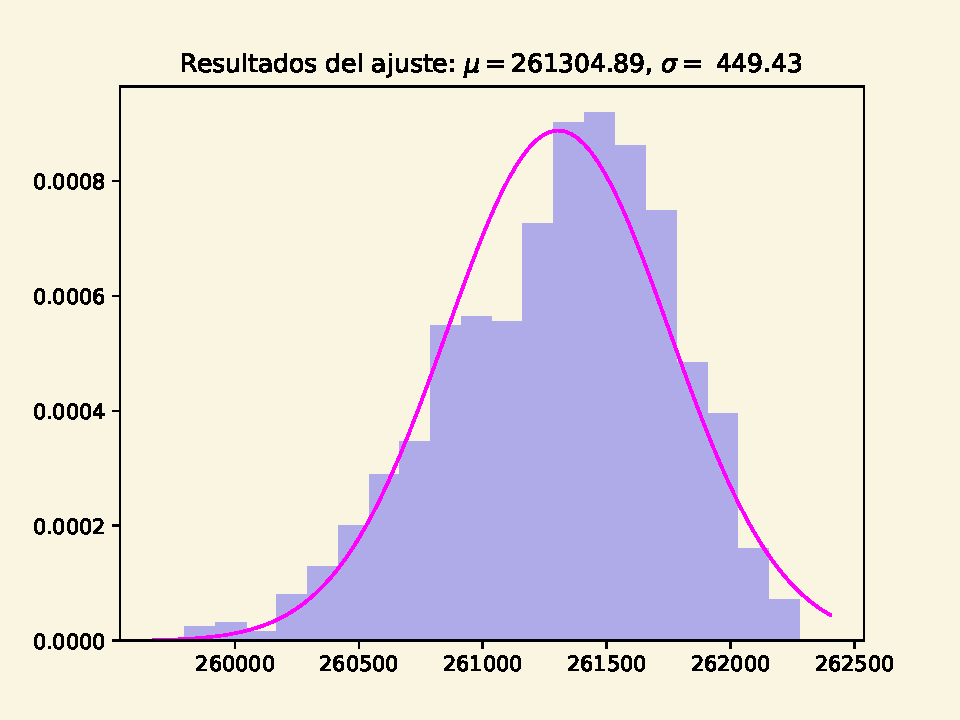
\includegraphics[scale=0.8]{histogram_depths.pdf}
					\caption{Histograma de los datos obtenidos de la simulación.}
					\label{fig:Histograma}
				\end{figure}

				Por lo que la profundidad máxima que alcanza es de

				\begin{empheq}[box = \color{pinkwave}\fbox]{equation*}
					t_{\text{máx}} = \SI{261304.89}{\m}.
				\end{empheq}

				Y la distribución que sigue es una distribución normal o gaussiana.
			\end{solution}
		\end{enumerate}
	\end{exercise}
\end{document}
